%%%%%%%%%%%%%%%%%%%%%%%%%%%%%%%%%%%%%%%%%%%%%%%%%%%%%%%%%%%%%%%%%%%%%%
% How to use writeLaTeX:
%
% You edit the source code here on the left, and the preview on the
% right shows you the result within a few seconds.
%
% Bookmark this page and share the URL with your co-authors. They can
% edit at the same time!
%
% You can upload figures, bibliographies, custom classes and
% styles using the files menu.
%
% If you're new to LaTeX, the wikibook is a great place to start:
% http://en.wikibooks.org/wiki/LaTeX
%
%%%%%%%%%%%%%%%%%%%%%%%%%%%%%%%%%%%%%%%%%%%%%%%%%%%%%%%%%%%%%%%%%%%%%%
\documentclass{tufte-handout}

%\geometry{showframe}% for debugging purposes -- displays the margins

\usepackage{amsmath}

% Set up the images/graphics package
\usepackage{graphicx}
\setkeys{Gin}{width=\linewidth,totalheight=\textheight,keepaspectratio}
\graphicspath{{graphics/}}

\title{Stata Lab 5: Descriptive Statistics}
\author{DIME Analytics \\ dimeanalytics@worldbank.org}
% \date{24 January 2009}  % if the \date{} command is left out, the current date will be used

% The following package makes prettier tables.  We're all about the bling!
\usepackage{booktabs}

% The units package provides nice, non-stacked fractions and better spacing
% for units.
\usepackage{units}

% The fancyvrb package lets us customize the formatting of verbatim
% environments.  We use a slightly smaller font.
\usepackage{upquote}
\usepackage{fancyvrb}
\fvset{fontsize=\normalsize}
\renewcommand{\FancyVerbFormatLine}{\color{violet}}
\DefineShortVerb{\|}

% Small sections of multiple columns
\usepackage{multicol}

% Provides paragraphs of dummy text
\usepackage{lipsum}

% These commands are used to pretty-print LaTeX commands
\newcommand{\doccmd}[1]{\texttt{\textbackslash#1}}% command name -- adds backslash automatically
\newcommand{\docopt}[1]{\ensuremath{\langle}\textrm{\textit{#1}}\ensuremath{\rangle}}% optional command argument
\newcommand{\docarg}[1]{\textrm{\textit{#1}}}% (required) command argument
\newenvironment{docspec}{\begin{quote}\noindent}{\end{quote}}% command specification environment
\newcommand{\docenv}[1]{\textsf{#1}}% environment name
\newcommand{\docpkg}[1]{\texttt{#1}}% package name
\newcommand{\doccls}[1]{\texttt{#1}}% document class name
\newcommand{\docclsopt}[1]{\texttt{#1}}% document class option name

\begin{document}

\maketitle% this prints the handout title, author, and date

\begin{marginfigure}%
  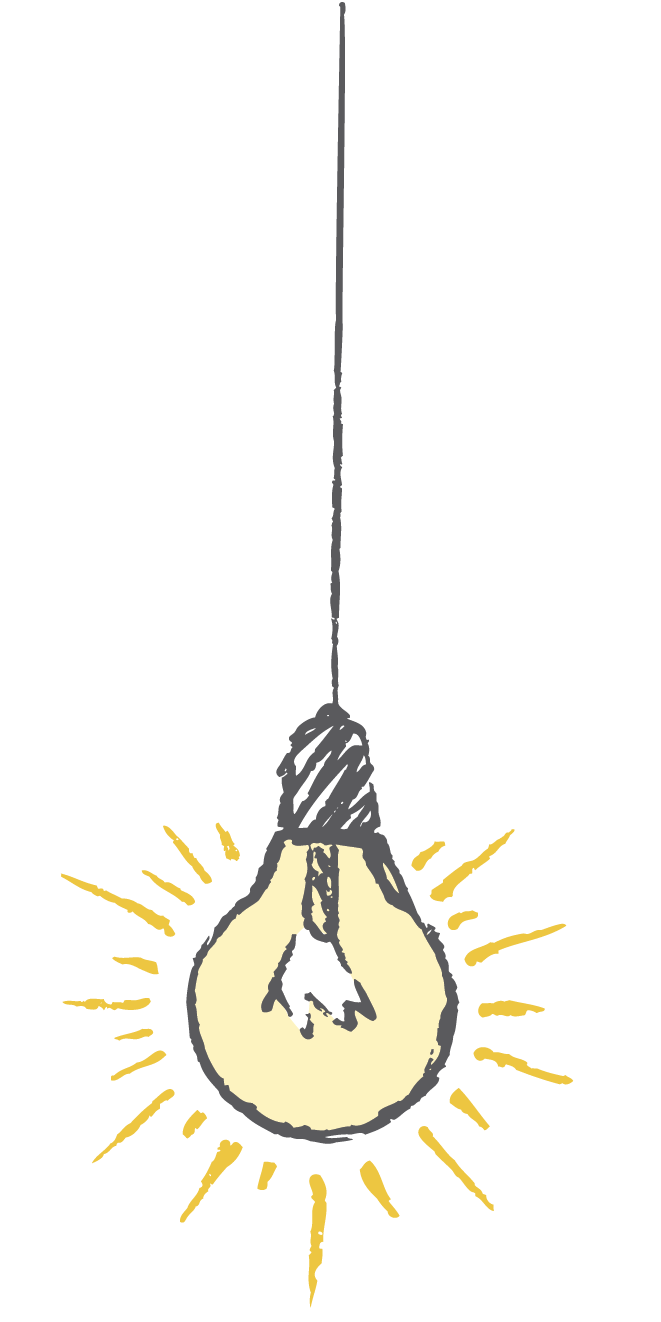
\includegraphics[width=\linewidth]{light.png}
\end{marginfigure}

\begin{abstract}
In this lab, we will learn to produce descriptive statistics in Stata.
These are numbers or figures that paint a picture of what a given dataset looks like.
We will also show you how to output simple balance tests and regressions.
These results begin to help us understand the important features of our dataset,
and can be useful in directing us towards areas for further analysis.

\bigskip\noindent \textbf{Exercise Objectives}:
\begin{enumerate}
  \item Learn how to produce and export tables of summary statistics
  \item Learn how to produce and export balance tables
  \item Learn how to produce and export simple regression tables
\end{enumerate}

\bigskip\noindent \textbf{Getting Started}:
\begin{enumerate}
 \item Open your |/DataWork/| folder for the full training. It should have subfolders for each of the Labs; if it does not, use |iefolder| to create the folder |/Lab5/| now.
 \item You will find a data file that we created in Lab 2, |hh_roster.dta| in the public Field Coordinator Training folder. Save this dataset to |/DataWork/Lab5/|.
 \item Install |sumstats| using |ssc install| (this command will only work on Stata 15.1 or greater). Install |esttab| and |outreg2| using |ssc install|.
\end{enumerate}
\end{abstract}

%\printclassoptions
\section{Producing summary statistics}

Create a new dofile and save it as |summary-statistics.do|.
We will look at control variables for outside income and food security:
|hh_fs_01|, |hh_fs_03|, |hh_fs_05|, |hh_inc_01|, and |hh_inc_02|.
For outcomes, we will use a takeup variable for LWH terracing income |hh_inc_12|;
and we will use another outcome variable for livestock sales, |hh_inc_08|.

Read the helpfile and use |sumstats| to summarize
the outcome and control variables for the dataset as a whole.
Display the number of observations, mean, median, standard deviation,
minimum and maximum values in the columns.
Then, create a second table displaying the same statistics
for control and treatment groups separately;
add a third panel showing these statistics only
for data that represents households using the |tag_hh| variable.

You can also use |putexcel| to accomplish similar tasks.
Try using |putexcel| in combination with |tabstat , save|:
\begin{Verbatim}[frame=leftline,numbers=left]
tabstat `controls' `outcome1' `outcome2' ///
  , save stats(N mean median sd min max)
mat results = r(StatTotal)' // Reformat results matrix

putexcel set "${Lab5}/summary-statistics-3.xlsx" , replace
putexcel A1 = mat(results , names)
\end{Verbatim}
When you are complete, your dofile might look like the one below.

\section{Producing balance tables}
Next, create a balance table using |iebaltab|.
This command is part of the |ietoolkit| package.
If you don’t yet have this package installed,
you can install it by typing |ssc install ietoolkit|.

Use |iebaltab| to run t-tests on the variables |hh_head_gender|,
|hh_hhsize|, and the |hh_inc_*| variables across treatment and control households.
Save this as |balance-1.xlsx|.
Then, add row labels using the variable labels,
and add a column for the total sample.
Save this as |balance-2.xlsx|.
Type |help iebaltab| for instructions about how to do this.
Don't use the |browse| option for now,
as it will clear the data you have in memory.
Finally, relabel the variables in your table manually;
and add an overall F-test for joint significance
of the differences; and treat missings as zeroes using |balmiss()|.
Save this as |balance-3.xlsx|.
When you are done, your dofile might look like the one below.

\section{Producing regression tables}
Most regression tables fall into one of two broad development stages.
In Stage One, you only care about making the information human-readable now,
and you are going to use those results to adjust the structure of the table repeatedly.
You may adjust the models and parameters, rename the rows and columns, delete or add lines;
but you will probably not finalize the output for a while.
Therefore, Stage One only requires you to export minimally formatted and annotated tables:
just enough to understand what your results are telling you.
This should not take long to implement, as formatting is usually the hardest part.
And really, you don't want to spend a lot of time making you table look nice,
if you may not even use it for the final output.

Two of the most commonly-used packages for writing tables, |estout| and |outreg2|,
are two of the top three most-downloaded packages from SSC.
Both of these can create simple tables in \LaTeX\ or Excel,
although they will not always look the nicest without formatting.
Exporting results to individual |.tex| files for each table and
importing them with |input| into a master |.tex| document
is the easiest way to create outputs when you are still making changes to the results. It will look like this:
\begin{Verbatim}
  {
\def\sym#1{\ifmmode^{#1}\else\(^{#1}\)\fi}
\begin{tabular}{l*{4}{c}}
\hline\hline
            &\multicolumn{1}{c}{(1)}&\multicolumn{1}{c}{(2)}&\multicolumn{1}{c}{(3)}&\multicolumn{1}{c}{(4)}\\
            &\multicolumn{1}{c}{hh\_inc\_08}&\multicolumn{1}{c}{hh\_inc\_12}&\multicolumn{1}{c}{hh\_inc\_08}&\multicolumn{1}{c}{hh\_inc\_08}\\
            &  b/\_star/se&  b/\_star/se&  b/\_star/se&  b/\_star/se\\
\hline
hh\_fs\_01    &  -2815.432 &   2983.739 &  -2420.588 &  -2420.588 \\
            &    6764.664&     5765.24&    6802.906&    6802.906\\
hh\_fs\_03    &  -7731.882 &   1962.582 &  -7157.081 &  -7157.081 \\
            &     5202.96&    6427.086&      5370.3&      5370.3\\
hh\_fs\_05    &-4781.896 \sym{*}&-10674 \sym{*}&-7352.576 \sym{**}&-7352.576 \sym{**}\\
            &    2301.591&    4287.071&    2733.488&    2733.488\\
hh\_inc\_01   &.0975817 \sym{**}&  -.0058587 &.0949967 \sym{**}&.0949967 \sym{**}\\
            &    .0360981&    .0052585&    .0349807&    .0349807\\
hh\_inc\_02   &.00104 \sym{***}&-.0000413 \sym{***}&.0010692 \sym{***}&.0010692 \sym{***}\\
            &    .0000572&    .0000102&    .0000495&    .0000495\\
hh\_treatment&            &            &-12401.8 \sym{*}&-12401.8 \sym{*}\\
            &            &            &    5249.326&    5249.326\\
\_cons      &13837.1 \sym{***}&11386.71 \sym{***}&20232.43 \sym{***}&20232.43 \sym{***}\\
            &    2578.852&    1796.649&    4414.977&    4414.977\\
\hline
\(N\)       &        3735&        3732&        3735&        3735\\
\hline\hline
\end{tabular}
}

\end{Verbatim}

\bigskip
\noindent{
\def\sym#1{\ifmmode^{#1}\else\(^{#1}\)\fi}
\begin{tabular}{l*{4}{c}}
\hline\hline
            &\multicolumn{1}{c}{(1)}&\multicolumn{1}{c}{(2)}&\multicolumn{1}{c}{(3)}&\multicolumn{1}{c}{(4)}\\
            &\multicolumn{1}{c}{hh\_inc\_08}&\multicolumn{1}{c}{hh\_inc\_12}&\multicolumn{1}{c}{hh\_inc\_08}&\multicolumn{1}{c}{hh\_inc\_08}\\
            &  b/\_star/se&  b/\_star/se&  b/\_star/se&  b/\_star/se\\
\hline
hh\_fs\_01    &  -2815.432 &   2983.739 &  -2420.588 &  -2420.588 \\
            &    6764.664&     5765.24&    6802.906&    6802.906\\
hh\_fs\_03    &  -7731.882 &   1962.582 &  -7157.081 &  -7157.081 \\
            &     5202.96&    6427.086&      5370.3&      5370.3\\
hh\_fs\_05    &-4781.896 \sym{*}&-10674 \sym{*}&-7352.576 \sym{**}&-7352.576 \sym{**}\\
            &    2301.591&    4287.071&    2733.488&    2733.488\\
hh\_inc\_01   &.0975817 \sym{**}&  -.0058587 &.0949967 \sym{**}&.0949967 \sym{**}\\
            &    .0360981&    .0052585&    .0349807&    .0349807\\
hh\_inc\_02   &.00104 \sym{***}&-.0000413 \sym{***}&.0010692 \sym{***}&.0010692 \sym{***}\\
            &    .0000572&    .0000102&    .0000495&    .0000495\\
hh\_treatment&            &            &-12401.8 \sym{*}&-12401.8 \sym{*}\\
            &            &            &    5249.326&    5249.326\\
\_cons      &13837.1 \sym{***}&11386.71 \sym{***}&20232.43 \sym{***}&20232.43 \sym{***}\\
            &    2578.852&    1796.649&    4414.977&    4414.977\\
\hline
\(N\)       &        3735&        3732&        3735&        3735\\
\hline\hline
\end{tabular}
}

\bigskip

In this exercise, you’ll build up a simple regression model and export it,
using these two commands, into both Excel and \LaTeX.
First, build up some regression models using |regress| and |estimates store|.
Use |regress| with each outcome on the control variables only;
then save the estimates using |estimates store|.
Next, do the same two regression model with the treatment variable and
the control variables and store that. Cluster at the household level.
Then, output these four regressions together using |estout| and |outreg2|,
as Excel files and as |.tex| files.
Feel free to explore the formatting options for both.

Thanks to the template creators.\cite{tuftelatex}

\bibliography{sample-handout}
\bibliographystyle{plainnat}

\newpage

\begin{figure*}[h]
{\setstretch{0.7}
\VerbatimInput[frame=lines,numbers=left,label=summary-statistics.do]
{../DataWork/Lab5/summary-statistics.do}}
\end{figure*}

\begin{figure*}[h]
{\setstretch{0.7}
\VerbatimInput[frame=lines,numbers=left,label=balance-table.do]
{../DataWork/Lab5/balance-table.do}}
\end{figure*}

\begin{figure*}[h]
{\setstretch{0.7}
\VerbatimInput[frame=lines,numbers=left,label=regressions.do]
{../DataWork/Lab5/regressions.do}}
\end{figure*}

\end{document}
